\begin{frame}[fragile]
    \frametitle{Architecture}
    \begin{figure}
        \includegraphics[scale=.21]{figures/architecture}
    \end{figure}
\end{frame}

\begin{frame}
  \frametitle{Une question}
    \alert{Where does the prime minister of the United Kingdom live?}
\end{frame}

\begin{frame}
 \frametitle{De la question à la forme normale}

\begin{center}
  \alert{Where does the prime minister of the United Kingdom live?}
\end{center}

\begin{figure}
 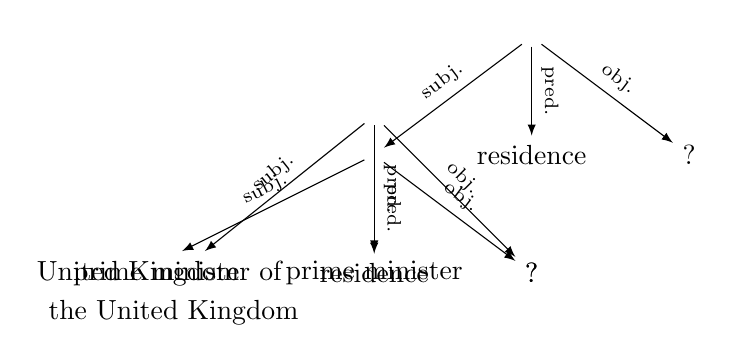
\begin{tikzpicture}
  \onslide<1>{
  \node (7) at (8,9) {$\triple$};
  \node (8) at (5.5,7) {prime minister of};
  \node (11) at (5.45,6.5) {the United Kingdom};
  \node (9) at (8,7) {residence};
  \node (10) at (10,7) {?};

  \draw[->, >=latex] (7) edge node[sloped, anchor=center, above] {\scriptsize{subj.}} (8);
  \draw[->, >=latex] (7) edge node[sloped, anchor=center, above] {\scriptsize{pred.}} (9);
  \draw[->, >=latex] (7) edge node[sloped, anchor=center, above] {\scriptsize{obj.}} (10);}
  
  \onslide<2>{  
  \node (0) at (10,10) {$\triple$};
  \node (1) at (10,8.5) {residence};
  \node (2) at (12,8.5) {?};
  \node (3) at (8,8.5) {$\triple$};
  \node (4) at (8,7) {prime minister};
  \node (5) at (5,7) {United Kingdom};
  \node (6) at (10,7) {?};

  \draw[->, >=latex] (0) edge node[sloped, anchor=center, above] {\scriptsize{obj.}} (2);
  \draw[->, >=latex] (0) edge node[sloped, anchor=center, above] {\scriptsize{pred.}} (1);
  \draw[->, >=latex] (0) edge node[sloped, anchor=center, above] {\scriptsize{subj.}} (3);
  \draw[->, >=latex] (3) edge node[sloped, anchor=center, above] {\scriptsize{subj.}} (5);
  \draw[->, >=latex] (3) edge node[sloped, anchor=center, above] {\scriptsize{obj.}} (6);
  \draw[->, >=latex] (3) edge node[sloped, anchor=center, above] {\scriptsize{pred.}} (4);}
 \end{tikzpicture}
\end{figure}

\end{frame}

\begin{frame}
   \frametitle{Extraction de la réponse : Wikidata}

    Wikidata ?
    \begin{itemize}
        \item \alert{\url{http://www.wikidata.org}}
        \item Une base de \alert{connaissance libre}
        \item \alert{Multilingue}
    \end{itemize}
\end{frame}

\begin{frame}
  \frametitle{Extraction de la réponse : Wikidata}

\begin{figure}
 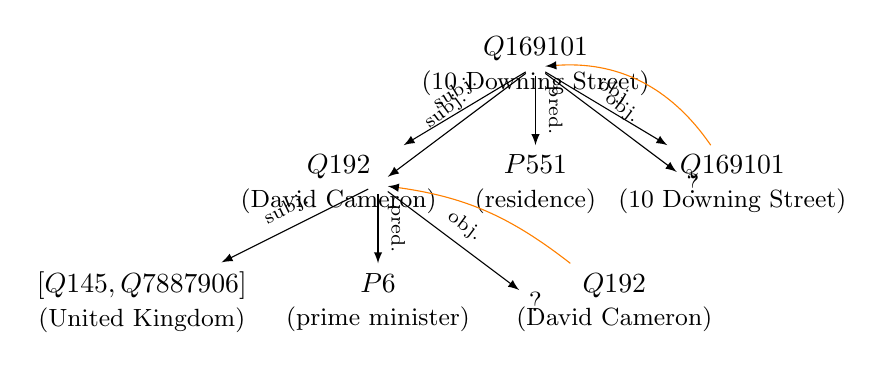
\begin{tikzpicture}
  \onslide<1-4>{\node (0) at (10,10) {$\triple$};}
  \onslide<1-4>{\node (1) at (10,8.5) [align=center] {$P551$\\{\small (residence)}};}
  \onslide<1-3>{\node (2) at (12,8.5) {?};}
  \onslide<1-2>{\node (3) at (8,8.5) {$\triple$};}
  \onslide<1-2>{\node (4) at (8,7) [align=center] {$P6$\\{\small (prime minister)}};}
  \onslide<1-2>{\node (5) at (5,7) [align=center] {$\left[Q145, Q7887906\right]$\\{\small (United Kingdom)}};}
  \onslide<1>{\node (6) at (10,7) {?};}

  \onslide<1-4>{\draw[->, >=latex] (0) edge node[sloped, anchor=center, above] {\scriptsize{pred.}} (1);}
  \onslide<1-3>{\draw[->, >=latex] (0) edge node[sloped, anchor=center, above] {\scriptsize{obj.}} (2);}
  \onslide<1-2>{\draw[->, >=latex] (0) edge node[sloped, anchor=center, above] {\scriptsize{subj.}} (3);}
  \onslide<1-2>{\draw[->, >=latex] (3) edge node[sloped, anchor=center, above] {\scriptsize{subj.}} (5);}
  \onslide<1-2>{\draw[->, >=latex] (3) edge node[sloped, anchor=center, above] {\scriptsize{obj.}} (6);}
  \onslide<1-2>{\draw[->, >=latex] (3) edge node[sloped, anchor=center, above] {\scriptsize{pred.}} (4);}
  
  \onslide<2>{\node (7) at (11,7) [align=center] {\alert{$Q192$}\\\alert{\small (David Cameron)}};}
  \onslide<3-4>{\node (8) at (7.5,8.5) [align=center] {\alert{$Q192$}\\\alert{\small (David Cameron)}};}
  \onslide<4>{\node (9) at (12.5,8.5) [align=center] {\alert{$Q169101$}\\\alert{\small (10 Downing Street)}};}
  \onslide<5>{\node (10) at (10,10) [align=center] {\alert{$Q169101$}\\\alert{\small (10 Downing Street)}};}

  \onslide<3-4>{\draw[->, >=latex] (0) edge node[sloped, anchor=center, above] {\scriptsize{subj.}} (8);}
  \onslide<4>{\draw[->, >=latex] (0) edge node[sloped, anchor=center, above] {\scriptsize{obj.}} (9);}

  \onslide<2>{\draw[->, >=latex] [draw=orange] [bend right=15, above] (7) edge (3);}
  \onslide<4>{\draw[->, >=latex] [draw=orange] [bend right, above] (9) edge (0);}
 \end{tikzpicture}
\end{figure}
\end{frame}


\begin{frame}
    \frametitle{Résultat final}
    \includegraphics[width=\linewidth]{figures/residence-prime-minister.png}
\end{frame}

\begin{frame}
    \frametitle{Recherche simple}
    \includegraphics[width=\linewidth]{figures/10-downing-street.png}
\end{frame}

\begin{frame}
    \frametitle{Math}
    TODO
\end{frame}
